\documentclass[9pt,a4paper]{article}

% --- Compiler: unbedingt XeLaTeX oder LuaLaTeX verwenden! ---
\usepackage{fontspec}
\setmainfont{SegoeUI}[
    Path = Fonts/,
    Extension = .ttf,
    UprightFont = *,
    BoldFont = *b,
    ItalicFont = *i,
    BoldItalicFont = *z
] % muss lokal installiert sein (System-Schriftart)
% Seitenränder

\usepackage[margin=2.5cm]{geometry}
\usepackage{titling}
\setlength{\droptitle}{-1.06cm}
\pretitle{\centering}
\posttitle{\par\vskip 9.5pt}
\preauthor{\par\centering\fontsize{10pt}{14.4pt}\selectfont}
\postauthor{\par}
\predate{}\postdate{}

\usepackage{setspace}
\usepackage{graphicx}
\usepackage{float}
\usepackage{lipsum}
\usepackage[dvipsnames]{xcolor}
\definecolor{gfaiblau}{HTML}{23355D}
\usepackage{sectsty}
\usepackage{hyperref}
\usepackage{booktabs,multicol,multirow,tabularx,array}    
\usepackage[withpage]{acronym}
\usepackage{cite}
\usepackage{shortvrb}
\usepackage{pdflscape}

\fontsize{9pt}{12pt}\selectfont

\subsectionfont{\centering\color{gfaiblau}\fontsize{10pt}{12pt}\selectfont\bfseries}
\sectionfont{\centering\color{gfaiblau}\fontsize{10pt}{12pt}\selectfont\bfseries}
\makeatletter
\renewcommand{\@seccntformat}[1]{\csname the#1\endcsname\hspace{0.3em}}
\renewcommand\normalsize{\@setfontsize\normalsize{9pt}{14.4pt}}
\renewcommand\section{\@startsection{section}{1}{\z@}%
      {-3.5ex \@plus -1ex \@minus -.2ex}{3.4ex \@plus.2ex}%
      {\normalfont\Large\bfseries\SS@sectfont}}
\renewcommand{\figurename}{Fig.}
\setlength{\abovecaptionskip}{-3pt}
\makeatother
\normalsize
\newlength{\preSecSkip}
\setlength{\preSecSkip}{11pt}
\let\oldsection\section
\renewcommand{\section}{\vspace*{\preSecSkip}\oldsection}

\title{\color{Black}{\bfseries\fontsize{12pt}{14pt}\selectfont Title}}
\author{%
{Name, first Author}$^{1}$, {Name, second Author}$^{2}$ \\
$^1$Institute, address, email address, web \\
$^2$Institute, address, email address, web
}
\pagestyle{empty}

\begin{document}

\date{}
\maketitle
\thispagestyle{empty}
\vspace{9pt}
\noindent
{\fontsize{9pt}{14.4pt}\selectfont
{\bfseries\color{gfaiblau}\fontsize{10pt}{14.4pt}\selectfont Abstract:}
Please insert your abstract here. This text is laid out in justified text. nis et laceptisi voluptatis et hicae nonsed quam, vellaceperae nobit ab id quae volut min nonsed molupta taspis et mo officidelita soloritatist faceaquatem quias autatiaspis es dolorem ra quae non rectur si solorerovid qui doluptam doloribus et ute di reic
}

\vspace{15pt}
{\centering
\fontsize{9pt}{14.4pt}\selectfont
{\bfseries\color{gfaiblau}\fontsize{10pt}{14.4pt}\selectfont Keywords:}
example; example; example\par
}

\section{Subheadline / Chapter heading (Segoe UI, Bold, 10 pt, dark blue)}
Here follows the body text of your academic work. ictata quam, sed esti conemoluptae eatent paris sunt dem earunt es expla intia ped quidem simpelliquae nis et laceptisi voluptatis et hicae nonsed quam, vellaceperae nobit ab id quae volut min nonsed molupta taspis et mo officidelita soloritatist faceaquatem quias autatiaspis es dolorem ra quae non rectur si solorerovid qui doluptam doloribus et ute di reic tem dolorporest, acia dolesti oressimint eatio entium quodici enist, explia nis es doluptaquas adi doluptam voloreh endendunt labo. Pit atiis due. \cite{Literature}
\begin{figure}[H]
    \centering
    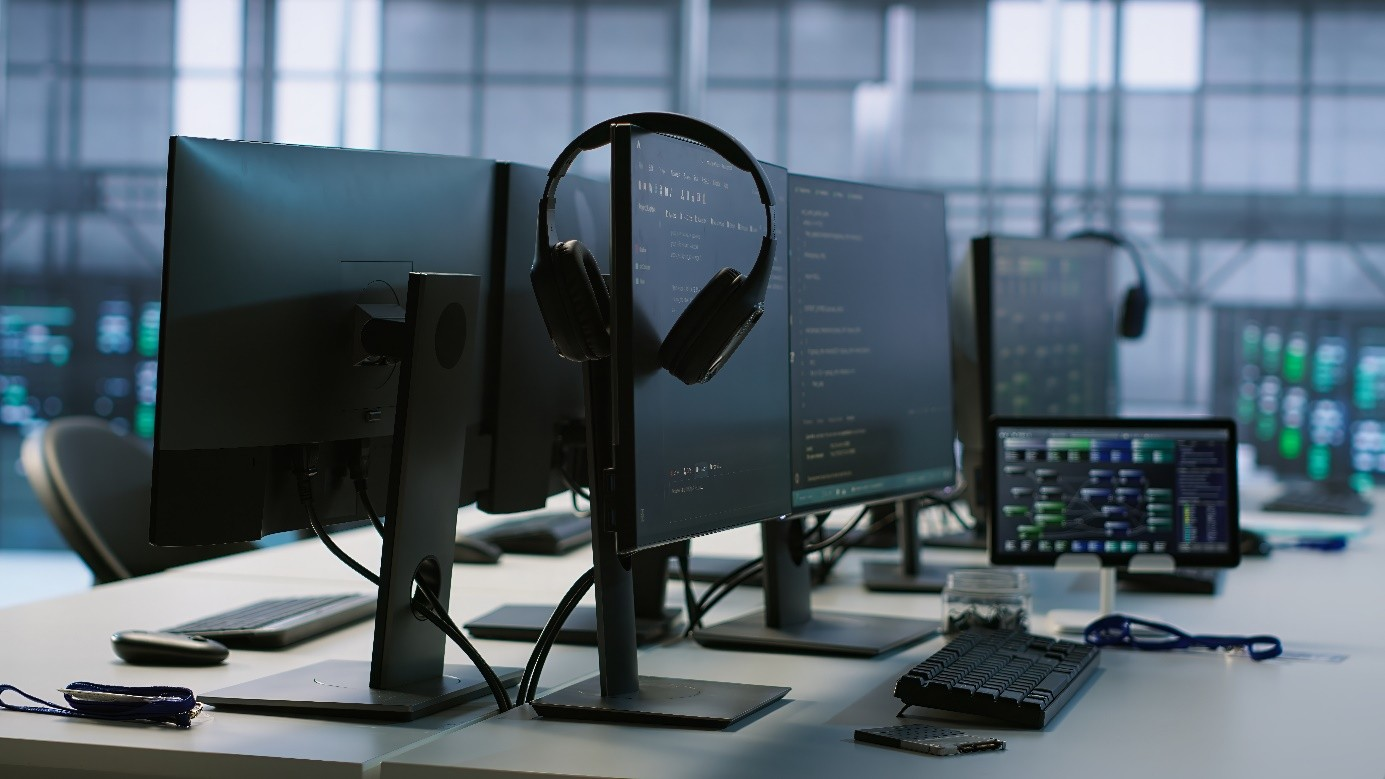
\includegraphics[width= \linewidth]{Images/Beispielbild.jpg}
    \caption{Caption (Center the image.)}
    \label{fig:enter-label}
\end{figure}




\bibliographystyle{ieeetr}
\bibliography{citing}
\end{document}
